\pdfoutput=1
\documentclass[12pt]{article}
\usepackage{graphicx}
\usepackage{subcaption}
\usepackage{amssymb}
\usepackage{amsmath}
\usepackage{amsfonts}
\usepackage{multirow}
\usepackage{appendix}

%\usepackage{color}
\usepackage{xcolor}
\usepackage{url}
%\usepackage{cancel}
\usepackage{ulem}
\usepackage{float}
%black, blue, brown, cyan, darkgray, gray, green, lightgray, lime,
%magenta, olive, orange, pink, purple, red, teal, violet, white, yellow.
%\usepackage{bm}
\usepackage{float}
%\usepackage{jheppub}

\usepackage{pifont}% http://ctan.org/pkg/pifont
\newcommand{\cmark}{\ding{51}}%
\newcommand{\xmark}{\ding{55}}%

\usepackage{soul}
\usepackage[english]{babel}
\usepackage[T1]{fontenc}
\usepackage{lmodern}
 % Einstellungen, wenn man deutsch schreiben will, z.B. Trennregeln
\usepackage[utf8]{inputenc}  % f??r Unix-Systeme
  % erm??glicht die direkte Eingabe von Umlauten und ??
  % evt. obige Zeile ersetzen durch
  % \usepackage[utf8]{inputenc}
  % \usepackage[ansinew]{inputenc}  % f??r Windows
  % \usepackage[applemac]{inputenc} % f??r den Mac
\usepackage{bbm}


\usepackage{hyperref}
\hypersetup{
  colorlinks   = true, %Colours links instead of ugly boxes
  urlcolor     = blue, %Colour for external hyperlinks
  linkcolor    = black, %Colour of internal links
  citecolor   = black %Colour of citations
}


\usepackage[numbers,sort&compress]{natbib}
%\bibliographystyle{JHEP}
\bibliographystyle{kp}


%\usepackage{geometry}
%\geometry{textheight=230mm,textwidth=165mm,footskip=20mm}



\graphicspath{{plots/}}

%\hypersetup{linktocpage}
%\voffset -1cm
%\hoffset 0.1cm
% \textwidth 16.5cm
% \textheight 21.5cm
% %\topmargin -0.5cm
% \renewcommand{\baselinestretch}{1.30}                                
% \newcommand{\mnote}[1]{\marginpar{%                               
%         \vskip-\baselineskip                                               
%         \raggedright\footnotesize                                          
%         \itshape\hrule\smallskip\tiny\bf{#1}\par\smallskip\hrule}}
% \def\hlite#1{\textcolor{blue}{\textsf{#1}}}
% \def\hlitebrown#1{\textcolor{brown}{\textsf{#1}}}
% \def\hlitered#1{\textcolor{red}{\textsf{#1}}}
 \def\is#1{\textcolor{blue}{#1}}

%==============================================================================
%\input{just_def.tex}

\newcommand{\lsim}
{\;\raisebox{-.3em}{$\stackrel{\displaystyle <}{\sim}$}\;}
\newcommand{\gsim}
{\;\raisebox{-.3em}{$\stackrel{\displaystyle >}{\sim}$}\;}

\newcommand\Code[1]{\ensuremath{\texttt{#1}}}
\newcommand\Var[1]{\ensuremath{\mathit{#1}}}
\newcommand\Vi{\Var{i}}
\newcommand\Vj{\Var{j}}
\newcommand\Vt{\Var{t}}
\newcommand\Vg{\Var{g}}
\newcommand\Vs{\Var{s}}

\newcommand\al{\alpha}
\newcommand\be{\beta}
\newcommand\tb{\tan\beta}
\newcommand\TB{t_\beta}
\newcommand\SB{s_\beta}
\newcommand\CB{c_\beta}
\newcommand\CBB{c_{2\beta}}
\newcommand\SA{s_\alpha}
\newcommand\CA{c_\alpha}
\newcommand\CBA{c_{\beta - \alpha}}
\newcommand\SBA{s_{\beta - \alpha}}
\newcommand\CAB{c_{\alpha + \beta}}
\newcommand\SAB{s_{\alpha + \beta}}

\newcommand\LP{\left(}
\newcommand\RP{\right)}
\newcommand\LB{\left[}
\newcommand\RB{\right]}
\newcommand\LV{\left\{}
\newcommand\RV{\right\}}
\newcommand\ra{\rightarrow}
\newcommand\tenp[1]{\times 10^{#1}}

\renewcommand\Re{\mathop{\mathrm{Re}}}
\renewcommand\Im{\mathop{\mathrm{Im}}}
\newcommand\ReTilde{\mathop{\widetilde{\mathrm{Re}}}}
\newcommand\ReDiag{\mathop{%
  \raise .5pt\hbox{[}%
  \widetilde{\mathrm{Re}}%
  \raise .5pt\hbox{]}}}
\newcommand\ReOffDiag{\mathop{%
  \raise .5pt\hbox{$\llbracket$}%
  \widetilde{\mathrm{Re}}%
  \raise .5pt\hbox{$\rrbracket$}}}
\newcommand\SE[1]{\Sigma_{#1}}
\newcommand\OS{\mathrm{OS}}
\newcommand\DRbar{\ensuremath{\smash{\overline{\mathrm{DR}}}}}
\newcommand\MSbar{\ensuremath{\overline{\mathrm{MS}}}}
\newcommand\matr[1]{\mathbf{#1}}
\newcommand\mati[1]{\bigl(#1\bigr)}
\newcommand\unity{\mathrm{1\mskip-4.25mu l}}
\newcommand\ddiv{\bigr|_{\mathrm{div}}}
\newcommand\Ddiv{\Bigr|_{\mathrm{div}}}
\newcommand\cMt{{\cal M}_{\text{tree}}}
\newcommand\cMl{{\cal M}_{\text{1-loop}}}
\newcommand\cL{{\cal L}}

\newcommand\SW{s_\mathrm{w}}
\newcommand\CW{c_\mathrm{w}}
\newcommand\MW{M_W}
\newcommand\MZ{M_Z}
\newcommand\Mh{M_h}
\newcommand\MH{M_H}
\newcommand\MA{M_A}
\newcommand\MHp{M_{H^\pm}}
\newcommand{\mphi}{m_\phi}
\newcommand\mf[1]{m_{f_{#1}}}
\newcommand\mb{m_b}
\newcommand\mt{m_t}
\newcommand\Ab{A_b}
\newcommand\At{A_t}
\newcommand\Atau{A_\tau}
\newcommand\Amu{A_\mu}
\newcommand\Ae{A_e}

\newcommand\Sf{\tilde f}
\newcommand\Sfp{\tilde f^\prime}
\newcommand\msf[1]{m_{\Sf_{#1}}}
\newcommand\msfp[1]{m_{\Sfp_{#1}}}
\newcommand\Sn{\tilde\nu}
\newcommand\Sl{\tilde l}
\newcommand\sle[1]{\tilde l_{#1}}
\newcommand\Slpm{\tilde l^\pm}
\newcommand\msn[1]{m_{\Sn_{#1}}}
\newcommand\Sel[1]{\tilde e_{#1}}
\newcommand\Smu[1]{\tilde \mu_{#1}}
\newcommand\Fe{\mathrm{e}}
\newcommand\mfe[1]{m_{\Fe_{#1}}}
\newcommand\mse[1]{m_{\Sel{#1}}}
\newcommand\msl[1]{m_{\Sl_{#1}}}
\newcommand\Su{\mathrm{\tilde u}}
\newcommand\Fu{\mathrm{u}}
\newcommand\mfu[1]{m_{\Fu_{#1}}}
\newcommand\msu[1]{m_{\Su_{#1}}}
\newcommand\Sd{\mathrm{\tilde d}}
\newcommand\Fd{\mathrm{d}}
\newcommand\mfd[1]{m_{\Fd_{#1}}}
\newcommand\msd[1]{m_{\Sd_{#1}}}
\newcommand\hmsu[1]{\hat m_{\Su_{#1}}}
\newcommand\hmsd[1]{\hat m_{\Sd_{#1}}}
\newcommand\Stau[1]{{\tilde\tau_{#1}}}
\newcommand\stau{\tilde \tau}
\newcommand\Stop[1]{{\tilde t_{#1}}}
\renewcommand\stop{\tilde t}
\newcommand\Sbot[1]{{\tilde b_{#1}}}
\newcommand\sbot{\tilde b}

\newcommand\mL{m_{\tilde l_L}}
\newcommand\mR{m_{\tilde l_R}}
\newcommand\msnu{m_{\tilde \nu_l}}

\newcommand\cind{c^{\phantom{\prime}}}
\newcommand\cpri{c^\prime}
\newcommand\nind{n^{\phantom{\prime}}}
\newcommand\npri{n^\prime}
\newcommand\sind{s^{\phantom{\prime}}}
\newcommand\spri{s^{\prime}}
\newcommand\dZ[1]{\delta Z_{#1}}
\newcommand\dZm[1]{\delta\matr{Z}_{#1}}
\newcommand\dbZm[1]{\delta\matr{\breve Z}_{#1}}
\newcommand\dBZm[1]{\delta\matr{\breve{\bar Z}}{}_{#1}}

\newcommand\gl{{\tilde g}}
\newcommand\mgl{m_\gl}
\newcommand\phigl{\varphi_\gl}
\newcommand\dTB{\delta\TB}
\newcommand\ino[1]{\tilde\chi_{#1}}
\newcommand\mino[1]{m_{\ino{#1}}}
\newcommand\chapm[1]{\ino{#1}^\pm}
\newcommand\champ[1]{\ino{#1}^\mp}
\newcommand\chap[1]{\ino{#1}^+}
\newcommand\cham[1]{\ino{#1}^-}
\newcommand\cha{\chapm}
\newcommand\mcha[1]{m_{\chapm{#1}}}
\newcommand\mchap[1]{m_{\ino{#1}^+}}
\newcommand\mcham[1]{m_{\ino{#1}^-}}
\newcommand\neu[1]{\ino{#1}^0}
\newcommand\mneu[1]{m_{\neu{#1}}}

\newcommand\refeq[1]{Eq.~(\ref{#1})}
\newcommand\refeqs[1]{Eqs.~(\ref{#1})}
\newcommand\refta[1]{Tab.~\ref{#1}}
\newcommand\refse[1]{Sect.~\ref{#1}}
\newcommand\refses[1]{Sects.~\ref{#1}}
\newcommand\citere[1]{Ref.~\cite{#1}}
\newcommand\citeres[1]{Refs.~\cite{#1}}

\newcommand\lbrac{\symbol{123}}
\newcommand\rbrac{\symbol{125}}
\newcommand\Brac[1]{\lbrac#1\rbrac}
\newcommand\uscore{\symbol{95}}
\newcommand\eg{e.g.}
\newcommand\ie{i.e.\ }
\newcommand\wrt{w.r.t.\ }

\newcommand{\SM}{\mathrm{SM}}
\newcommand{\MSSM}{\mathrm{MSSM}}
\newcommand{\NMSSM}{\mathrm{NMSSM}}
\newcommand{\mnSSM}{\ensuremath{\mu\nu\mathrm{SSM}}}

\newcommand\trans{T}
\newcommand{\CP}{{\cal CP}}
\newcommand{\cp}{{\CP}}
\newcommand{\os}{\mathrm{os}}
\newcommand{\wtre}{\widetilde\Re}
\newcommand{\wtim}{\widetilde\Im}
\newcommand{\onel}{one-loop}
\newcommand{\tev}{\,\, \mathrm{TeV}}
\newcommand{\gev}{\,\, \mathrm{GeV}}
\newcommand{\mev}{\,\, \mathrm{MeV}}
\newcommand{\kev}{\,\, \mathrm{keV}}
\newcommand{\Hpm}{H^\pm}
\newcommand{\He}{h_1}
\newcommand{\Hz}{h_2}
\newcommand{\Hd}{h_3}

\newcommand{\eehh}{e^+e^- \to h_i h_j}
\newcommand{\eehZ}{e^+e^- \to h_i Z}
\newcommand{\eehga}{e^+e^- \to h_i \ga}

\newcommand{\eeHH}{e^+e^- \to H^+ H^-}
\newcommand{\eeHW}{e^+e^- \to H^{\pm} W^{\mp}}
\newcommand{\eeHpWm}{e^+e^- \to H^{+} W^{-}}
\newcommand{\eeHmWp}{e^+e^- \to H^{-} W^{+}}

\newcommand{\eecc}{\ensuremath{e^+e^- \to \chapm{c} \champ{\cpri}}}
\newcommand{\eecece}{e^+e^- \to \chap1 \cham1}
\newcommand{\eececz}{e^+e^- \to \chapm1 \champ2}
\newcommand{\eeczcz}{e^+e^- \to \chap2 \cham2}
\newcommand{\eecmcp}{e^+e^- \to \cham{c} \chap{\cpri}}
\newcommand{\eecpcm}{e^+e^- \to \chap{c} \cham{\cpri}}
\newcommand{\eecepczm}{e^+e^- \to \chap1 \cham2}
\newcommand{\eecemczp}{e^+e^- \to \cham1 \chap2}
\newcommand{\eeczpcem}{e^+e^- \to \chap2 \cham1}

\newcommand{\eenn}{\ensuremath{e^+e^- \to \neu{n} \neu{\npri}}}
\newcommand{\eenene}{e^+e^- \to \neu1 \neu1}
\newcommand{\eenznz}{e^+e^- \to \neu2 \neu2}
\newcommand{\eendnd}{e^+e^- \to \neu3 \neu3}
\newcommand{\eenvnv}{e^+e^- \to \neu4 \neu4}
\newcommand{\eenenz}{e^+e^- \to \neu1 \neu2}
\newcommand{\eenend}{e^+e^- \to \neu1 \neu3}
\newcommand{\eenenv}{e^+e^- \to \neu1 \neu4}
\newcommand{\eenznd}{e^+e^- \to \neu2 \neu3}
\newcommand{\eenznv}{e^+e^- \to \neu2 \neu4}
\newcommand{\eendnv}{e^+e^- \to \neu3 \neu4}

\newcommand{\eeSlSl}{\ensuremath{e^+e^- \to \Sl_{gs} \Sl_{gs^{\prime}}}}
\newcommand{\eeSeSe}{\ensuremath{e^+e^- \to \Se^{\pm}_{gs} \Se^{\mp}_{gs^{\prime}}}}
\newcommand{\eeSeeSee}{\ensuremath{e^+e^- \to \tilde{e}^+_1 \tilde{e}^-_1}}
\newcommand{\eeSeeSez}{\ensuremath{e^+e^- \to \tilde{e}^{\pm}_1 \tilde{e}^{\mp}_2}}
\newcommand{\eeSezSez}{\ensuremath{e^+e^- \to \tilde{e}^+_2 \tilde{e}^-_2}}
\newcommand{\eeSmeSme}{\ensuremath{e^+e^- \to \tilde{\mu}^+_1 \tilde{\mu}^-_1}}
\newcommand{\eeSmeSmz}{\ensuremath{e^+e^- \to \tilde{\mu}^{\pm}_1 \tilde{\mu}^{\mp}_2}}
\newcommand{\eeSmzSmz}{\ensuremath{e^+e^- \to \tilde{\mu}^+_2 \tilde{\mu}^-_2}}
\newcommand{\eeSaeSae}{\ensuremath{e^+e^- \to \tilde{\tau}^+_1 \tilde{\tau}^-_1}}
\newcommand{\eeSaeSaz}{\ensuremath{e^+e^- \to \tilde{\tau}^{\pm}_1 \tilde{\tau}^{\mp}_2}}
\newcommand{\eeSazSaz}{\ensuremath{e^+e^- \to \tilde{\tau}^+_2 \tilde{\tau}^-_2}}
\newcommand{\eeSnSn}{\ensuremath{e^+e^- \to \Sn_{g} \Sn_{g}}}
\newcommand{\eeSneSne}{\ensuremath{e^+e^- \to \tilde{\nu}_e \tilde{\nu}_e}}
\newcommand{\eeSnmSnm}{\ensuremath{e^+e^- \to \tilde{\nu}_{\mu} \tilde{\nu}_{\mu}}}
\newcommand{\eeSnaSna}{\ensuremath{e^+e^- \to \tilde{\nu}_{\tau} \tilde{\nu}_{\tau}}}

\newcommand\hChaDecay{h_i \to \cham{c} \chap{\cpri}}
\newcommand\hchaechae{h_i \to \champ1 \chapm1}
\newcommand\hchaechaz{h_i \to \champ1 \chapm2}
\newcommand\hchazchaz{h_i \to \champ2 \chapm2}
\newcommand\hNeuDecay{h_i \to \neu{n} \neu{\npri}}
\newcommand\hneueneue{h_i \to \neu1 \neu1}
\newcommand\hneuzneuz{h_i \to \neu2 \neu2}
\newcommand\hneudneud{h_i \to \neu3 \neu3}
\newcommand\hneuvneuv{h_i \to \neu4 \neu4}
\newcommand\hneueneuz{h_i \to \neu1 \neu2}
\newcommand\hneueneud{h_i \to \neu1 \neu3}
\newcommand\hneueneuv{h_i \to \neu1 \neu4}
\newcommand\hneuzneud{h_i \to \neu2 \neu3}
\newcommand\hneuzneuv{h_i \to \neu2 \neu4}
\newcommand\hneudneuv{h_i \to \neu3 \neu4}

\newcommand\hzstst{h_2 \to \Stop1 \Stop2, \Stop2 \Stop1}
\newcommand\hdstst{h_3 \to \Stop1 \Stop2, \Stop2 \Stop1}
\newcommand\hnstst{h_n \to \Stop1 \Stop2, \Stop2 \Stop1}
\newcommand\hzsbsb{h_2 \to \Sbot1 \Sbot2, \Sbot2 \Sbot1}
\newcommand\hnsbsb{h_n \to \Sbot1 \Sbot2, \Sbot2 \Sbot1}
\newcommand\hnstaustau{h_n \to \Stau1 \Stau2, \Stau2 \Stau1}
\newcommand\Hpdecay{H^+ \to \neu{n} \chap{c}}
\newcommand\Hmdecay{H^- \to \neu{n} \cham{c}}
\newcommand\HpmDecay{H^\pm \to \neu{n} \chapm{c}}
\newcommand\decayxy{H \to \text{xy}}
\newcommand\edz{\tfrac{1}{2}}
\newcommand\FA{\texttt{FeynArts}}
\newcommand\FC{\texttt{FormCalc}}
\newcommand\LT{\texttt{LoopTools}}
\newcommand\FH{\texttt{FeynHiggs}}
\newcommand\fh{\texttt{FeynHiggs}}
\newcommand\FT{\texttt{FeynTools}}
\newcommand\MO{\texttt{MicrOMEGAs}}
\newcommand\CM{\texttt{CheckMATE}}
\newcommand\HDECAY{\texttt{HDECAY}}
\newcommand\Sq{{\tilde q}}
\newcommand\msq[1]{m_{\Sq_{#1}}}
\newcommand\Mt{\tilde{M}}
\newcommand\pb{\ensuremath{\mbox{pb}}}
\newcommand\fb{\ensuremath{\mbox{fb}}}
\newcommand\ab{\ensuremath{\mbox{ab}}}
\newcommand\ipb{\ensuremath{\pb^{-1}}}
\newcommand\ifb{\ensuremath{\fb^{-1}}}
\newcommand\iab{\ensuremath{\ab^{-1}}}

\newcommand\mh[1]{m_{h_{#1}}}
\newcommand\msqua[1]{m_{\tilde{q}_{#1}}}
\newcommand\mstop[1]{m_{\tilde{t}_{#1}}}
\newcommand\msbot[1]{m_{\tilde{b}_{#1}}}
\newcommand\msele[1]{m_{\tilde{e}_{#1}}}
\newcommand\msmu[1]{m_{\tilde{\mu}_{#1}}}
\newcommand\mstau[1]{m_{\tilde{\tau}_{#1}}}
\newcommand\msneu{m_{\tilde{\nu}_{e,\mu,\tau}}}
\newcommand\melesneu{m_{\tilde{\nu}_{e}}}
\newcommand\mmuesneu{m_{\tilde{\nu}_{\mu}}}
\newcommand\mtausneu{m_{\tilde{\nu}_{\tau}}}

\newcommand{\Scs}{$\mathcal S$}
\newcommand{\Sce}{S1}
\newcommand{\Scz}{S2}
\newcommand{\Scd}{S3}
\newcommand{\Scv}{S4}
\newcommand{\Scf}{S5}
\newcommand{\br}{\text{BR}}
\newcommand{\db}{\Delta_b}
\newcommand{\rmd}{\text{d}}

\newcommand{\sig}{\sigma}
\newcommand{\sigfull}{\sigma_{\text{full}}}
\newcommand{\sigtree}{\sigma_{\text{tree}}}
\newcommand{\sigloop}{\sigma_{\text{loop}}}
\newcommand{\sigweak}{\sigma_{\text{weak}}}
\newcommand{\sigvirt}{\sigma_{\text{virt}}}
\newcommand{\sigsoft}{\sigma_{\text{soft}}}
\newcommand{\sighard}{\sigma_{\text{hard}}}
\newcommand{\sigcoll}{\sigma_{\text{coll}}}

\newcommand{\StopL}{\tilde{t}_L}
\newcommand{\StopR}{\tilde{t}_R}
\newcommand{\Snutau}{\tilde{\nu}_\tau}

\newcommand{\phiAeg}{\varphi_{A_{\Fe_g}}}
\newcommand{\phiAug}{\varphi_{A_{\Fu_g}}}
\newcommand{\phiAdg}{\varphi_{A_{\Fd_g}}}

\def\order#1{\ensuremath{{\cal O}(#1)}}
\def\reffi#1{\mbox{Fig.~\ref{#1}}}
\def\reffis#1{\mbox{Figs.~\ref{#1}}}
\def\als{\alpha_s}
\def\alt{\alpha_t}
\def\alb{\alpha_b}
\def\Ga{\Gamma}
\def\ga{\gamma}
\def\De{\Delta}
\def\de{\delta}
\def\la{\lambda}
\def\phia{\varphi_{A}}
\def\phiAt{\varphi_{\At}}
\def\phiAtb{\varphi_{A_{t,b}}}
\def\phiAb{\varphi_{\Ab}}
\def\phiAtau{\varphi_{\Atau}}
\def\phiAmu{\varphi_{\Amu}}
\def\phiAe{\varphi_{\Ae}}
\def\phimu{\varphi_{\mu}}
\def\phiMe{\varphi_{M_1}}
\def\phiMz{\varphi_{M_2}}
\def\phigl{\varphi_{\gl}}
\def\MSUSY{M_{\text{SUSY}}}
\def\MSL{M_{\tilde L}}
\def\MSE{M_{\tilde E}}
\def\MSQ{M_{\tilde Q}}
\def\MSU{M_{\tilde U}}
\def\MSD{M_{\tilde D}}
\def\amususy{\ensuremath{a_\mu^{\rm SUSY}}}
\def\gmin2{\ensuremath{(g-2)_\mu}}
\def\amu{\ensuremath{a_\mu}}
\def \met  {\mbox{${E\!\!\!\!/_T}$}}
\newcommand{\ssi}{\ensuremath{\sig_p^{\rm SI}}}
\newcommand{\ssd}{\ensuremath{\sig_p^{\rm SD}}}
\newcommand{\Och}{\Omega_\chi h^2}

\definecolor{Orange}{named}{orange}
\definecolor{Purple}{named}{purple}
\definecolor{Lightblue}{cmyk}{0.9,0.1,0.1,0.3}
\definecolor{dgelborange}{cmyk}{0.,0.3,0.5, 0.}
\definecolor{Lila}{rgb}{0.5,0.,1}
\definecolor{Darkgreen}{rgb}{0.,.7,0.2}

\newcommand{\htr}[1]{{\color{red} #1}}
\newcommand{\htb}[1]{{\color{blue} #1}}
\newcommand{\htg}[1]{{\color{Darkgreen} #1}}
\newcommand{\hto}[1]{{\color{Orange}  #1}}
\newcommand{\htp}[1]{{\color{purple}  #1}}
\newcommand{\htbl}[1]{{\color{Lightblue}#1}}
\newcommand{\htlb}[1]{{\color{Lightblue}#1}}
\newcommand{\htgo}[1]{{\color{dgelborange}#1}}
\newcommand{\htli}[1]{{\color{Lila}#1}}
\newcommand{\htgray}[1]{{\color{black!40} #1}}
\newcommand{\htrd}[1]{\htr{\st{#1}}}
\newcommand{\htbd}[1]{\htb{\st{#1}}}
\newcommand{\htgd}[1]{\htg{\st{#1}}}
\newcommand{\htod}[1]{\hto{\st{#1}}}
\newcommand{\htpd}[1]{\htp{\st{#1}}}
\newcommand{\htlbd}[1]{\htlb{\st{#1}}}
\newcommand{\htgod}[1]{\htgo{\st{#1}}}
\newcommand{\htlid}[1]{\htli{\st{#1}}}
\def\grey#1{\special{ps: .6 setgray}#1\special{ps: 0 setgray}}


\newcommand{\sigmaobs}{\ensuremath{\sigma_{\rm obs}}}
\newcommand{\sigmaobsnfive}{\ensuremath{\sigma_{\rm obs,95}}}
\newcommand{\sigmanfive}{\ensuremath{\sigma_{\rm 95}}}
\newcommand{\deltanfive}{\ensuremath{\Delta_{\rm 95}}}
\newcommand{\sigmanfivepone}{\ensuremath{\sigma_{\rm 95,+1}}}
\newcommand{\deltanfivepone}{\ensuremath{\Delta_{\rm 95,+1}}}
\newcommand{\sigmanfiveptwo}{\ensuremath{\sigma_{\rm 95,+2}}}
\newcommand{\deltanfiveptwo}{\ensuremath{\Delta_{\rm 95,+2}}}
\newcommand{\deltaobsnfive}{\ensuremath{\Delta_{\rm obs,95}}}
\newcommand{\deltabkg}{\ensuremath{\Delta_{\rm bkg}}}
\newcommand{\deltaobs}{\ensuremath{\Delta_{\rm obs}}}




\oddsidemargin -0.5cm
\evensidemargin \oddsidemargin
\marginparwidth 68pt
\marginparsep 10pt
\topmargin 0cm
\headheight 0pt
\headsep 0pt
\footskip 1cm
\textheight 23cm
\textwidth 16.5cm
\columnsep 10pt
\columnseprule 0pt

\captionsetup{labelfont=bf, font=sf, size=small}
\renewcommand{\arraystretch}{1.2}

\allowdisplaybreaks
\sloppy

\hyphenation{Feyn-Arts process--indepen-dent}


%==============================================================================

\begin{document}
\thispagestyle{empty}


\def\thefootnote{\fnsymbol{footnote}}

\begin{flushright}
\mbox{}
%IFT--UAM/CSIC--20-077\\
%IPMU20-0057\\	
%arXiv:2006.15157 [hep-ph]
\end{flushright}

\vspace{0.5cm}

\begin{center}

{\large\sc
{\bf Possible New Higgs Bosons at \boldmath{$\sim 400 \gev$}
}}

\vspace{1cm}


{\sc
T.~Biek\"otter$^{1}$%
\footnote{email: thomas.biekoetter@desy.de}%
, A.~Grohsjean$^1$%
\footnote{email:alexander.grohsjean@desy.de}%
, S.~Heinemeyer$^{2,3,4}$%
\footnote{email: Sven.Heinemeyer@cern.ch}%
, V.M.~Lozano$^1$%
\footnote{email: victor.lozano@desy.de}%
,\\[.5em] C.~Schwanenberger$^1$%
\footnote{email: christian.schwanenberger@desy.de}%
~and G.~Weiglein$^{1}$%
\footnote{email: georg.weiglein@desy.de}%
}

\vspace*{.7cm}

{\sl
$^1$DESY, Notkestrasse 85, 22607 Hamburg, Germany

\vspace*{0.1cm}

$^2$IFT (UAM/CSIC), Universidad Aut\'onoma de Madrid, 
Cantoblanco, 28048, Spain

\vspace{0.1cm}

$^3$Campus of International Excellence UAM+CSIC, 
Cantoblanco, 28049, Madrid, Spain 

\vspace*{0.1cm}

$^4$Instituto de F\'isica de Cantabria (CSIC-UC), 
39005, Santander, Spain
}

\end{center}

\vspace*{0.1cm}

\begin{abstract}
\noindent
Several searches for Beyond the Standard Model (BSM) Higgs bosons at the
LHC show an excess at the level of $2-3\,\sig$ at a mass scale of
$\mphi \sim 400 \gev$. $\phi$ can either be a \cp-even Higgs boson,~$H$,
or a \cp-odd Higgs boson,~$A$. The respective search channels are
$pp \to H/A \to t \bar t$, $pp \to H/A \to \tau^+\tau^-$ and
$pp \to A \to Z h$, observed at CMS, ATLAS and ATLAS/CMS, respectively.
We derive/obtain best-fit cross sections and uncertainties for these excesses. 
Within the Next-to-2 Higgs Doublet Model (N2HDM) and the Next-to Minimal
Supersymmetric Standard Model (NMSSM) we analyze to what extent one, two
or three of these excesses can be fit simultaneously in the two models.
We find \ldots
\end{abstract}

%\pacs{}

\def\thefootnote{\arabic{footnote}}
\setcounter{page}{0}
\setcounter{footnote}{0}

\newpage


%%%%%%%%%%%%%%%%%%%%%%%%%%%%%%%%%%%%%%%%%%%%%%%%%%%%%%%%%%%%%%%%%%%%%%%%%%%%%%%
%%%%%%%%%%%%%%%%%%%%%%%%%%%%%%%%%%%%%%%%%%%%%%%%%%%%%%%%%%%%%%%%%%%%%%%%%%%%%%%


\section{Introduction}
\label{sec:intro}


\begin{itemize}

\item
Higgs is a big success, fits in the SM, but also in BSM models.

\item
Possible BSM models: 2HDM, N2HDM, \ldots, MSSM, NMSSM, \ldots

\item
LHC searches for BSM Higgs bosons. Excesses in various channels at the
$2-3\,\sig$ level. List channels etc.

\item
Main idea of the paper: check whether the N2HDM and NMSSM can accomodate
one, two or three of these excesses simultaneously.


\end{itemize}


%%%%%%%%%%%%%%%%%%%%%%%%%%%%%%%%%%%%%%%%%%%%%%%%%%%%%%%%%%%%%%%%%%%%%%%%%%%%%%%
%%%%%%%%%%%%%%%%%%%%%%%%%%%%%%%%%%%%%%%%%%%%%%%%%%%%%%%%%%%%%%%%%%%%%%%%%%%%%%%

\section{The Excesses}
\label{sec:excesses}

\noindent
More details on the excesses, best-fit cross sections and uncertainties,
$\chi^2$ function.

\begin{align}
\chi^2_{400} := \ldots
\label{chi400}
\end{align}

%%%%%%%%%%%%%%%%%%%%%%%%%%%%%%%%%%%%%%%%%%%%%%%%%%%%%%%%%%%%%%%%%%%%%%%%%%%%%%%
%%%%%%%%%%%%%%%%%%%%%%%%%%%%%%%%%%%%%%%%%%%%%%%%%%%%%%%%%%%%%%%%%%%%%%%%%%%%%%%

\section{The models}
\label{sec:models}

\noindent
We list the models and the codes that are used to evaluate them.\\
Maybe we can put some general considerations about which parameter
spaces are preferred to accomodate the excesses.


%%%%%%%%%%%%%%%%%%%%%%%%%%%%%%%%%%%%%%%%%%%%%%%%%%%%%%%%%%%%%%%%%%%%%%%%%%%%%%%


\subsection{The N2HDM}
\label{sec:n2hdm}

The simplest extension of the two Higgs doublet model (2HDM) that conserves $CP$ is achieved by adding a real scalar singlet Higgs field which gives rise to the so-called N2HDM. The scalar potential when the scalar singlet is added can be written as \cite{Chen:2013jvg,Muhlleitner:2016mzt}
\begin{align}
V&=m_{11}^2|\Phi_1|^2 + m_{22}^2|\Phi_2|^2 -m_{12}^2(\Phi_1^\dagger\Phi_2+ \text{h.c.}) +\frac{\lambda_1}{2}(\Phi_1^\dagger\Phi_1)^2+\frac{\lambda_2}{2}(\Phi_2^\dagger\Phi_2)^2 \notag \\
&+\lambda_3 (\Phi_1^\dagger\Phi_1)(\Phi_2^\dagger\Phi_2)+ \lambda_4(\Phi_1^\dagger\Phi_2)(\Phi_2^\dagger \Phi_1)+\frac{\lambda_5}{2}[(\Phi_1^\dagger\Phi_2)^2+\text{h.c.}]\notag\\
&+\frac{1}{2}m_S^2\Phi_S^2+\frac{\lambda_6}{8}\Phi_S^4+\frac{\lambda_7}{2}(\Phi_1^\dagger\Phi_1)\Phi_S^2+\frac{\lambda_8}{2}(\Phi_2^\dagger\Phi_2)\Phi_S^2,
\label{eq:n2hdmpotential}
\end{align}
the two $SU(2)_L$ doublets are $\Phi_1$ and $\Phi_2$ while $\Phi_S$ the real scalar singlet. One of the most problematic point when dealing with two Higgs doublet models is the appearance of flavour changing neutral currents (FCNC) at tree level. In order to avoid such phenomenon a $Z_2$ symmetry is imposed on the scalar potential in such a way that the scalar fields transform as
\begin{align}
\Phi_1\to\Phi_1,\,\, \Phi_2\to-\Phi_2,\,\, \Phi_S\to \Phi_S.
\end{align}
However, we can see from Eq.~\eqref{eq:n2hdmpotential} that this $Z_2$ symmetry is softly broken by the $m_{12}^2$ term. Despite this fact the extension of this symmetry to the Yukawa sector forbids strictly FCNSs at tree level.
In the Yukawa sector there are four variants of the N2HDM that depends on the configuration of the fermions with respect to the $Z_2$ symmetry. These four types are listed in Tab.~\ref{tab:yukawa}.

\begin{table}[ht]
  \begin{center}
    \begin{tabular}{l c c c}
    \hline
    &$u$-type& $d$-type& leptons\\
    \hline
    type I &$\Phi_2$&$\Phi_2$&$\Phi_2$\\
    type II &$\Phi_2$&$\Phi_1$&$\Phi_1$\\
    type III (lepton specific) &$\Phi_2$&$\Phi_2$&$\Phi_1$\\
    type IV (flipped) &$\Phi_2$&$\Phi_1$&$\Phi_2$\\
    \hline
    \end{tabular}
  \end{center}
\caption{Allowed fermion couplings in the four types of N2HDM.}
\label{tab:yukawa}
\end{table}

After electroweak symmetry breaking (EWSB) takes place, the scalar fields can be parameterised as
\begin{align}
\Phi_1=\left(
\begin{array}{c}
\phi_1^+\\
\frac{1}{\sqrt{2}}(v_1+\rho_1+i\eta_1)
\end{array}
\right),\,\,
\Phi_2=\left(
\begin{array}{c}
\phi_2^+\\
\frac{1}{\sqrt{2}}(v_2+\rho_2+i\eta_2)
\end{array}
\right),\,\,
\Phi_S=v_S+\rho_S,
\label{eq:EWSBfields}
\end{align}
where $v_1$, $v_2$ and $v_S$ are the real vacuum expectation values (vev) acquired by the fields $\Phi_1$, $\Phi_2$ and $\Phi_S$ respectively. We can define $\tan \beta=v_2/v1$ as it is usually done in the 2HDM. The configuration of the scalar fields after EWSB occurs, \textit{i.e.} Eq.~\eqref{eq:EWSBfields}, makes the charged and $CP$-odd Higgs sector remain unaltered with respecto to the 2HDM counterpart. However, that is not the case in the $CP$-even scalar sector due to the mixing of the three fields, $\rho_1$, $\rho_2$ and $\rho_S$. Such mixing configures the physical eigenstates under a $3\times 3$ orthogonal matrix, $R$, of the interaction basis, 
\begin{align}
\left(
\begin{array}{c}
h_1\\
h_2\\
h_3
\end{array}
\right)=R\left(
\begin{array}{c}
\rho_1\\
\rho_2\\
\rho_S
\end{array}
\right).
\end{align}
The subindex $i$, where $i=1,2,3$ respect the following order $m_{h_1}<m_{h_2}<m_{h_3}$ that we use in the rest of the paper. The form of the rotation matrix $R$ can be written as
\begin{align}
R=\left(
\begin{array}{ccc}
c_{\alpha_1}c_{\alpha_2}&s_{\alpha_1}c_{\alpha_2}&s_{\alpha_2}\\
-(c_{\alpha_1}s_{\alpha_2}s_{\alpha_3}+s_{\alpha_1}c_{\alpha_3})&c_{\alpha_1}c_{\alpha_3}-s_{\alpha_1}s_{\alpha_2}s_{\alpha_3}&c_{\alpha_2}s_{\alpha_3}\\
-c_{\alpha_1}s_{\alpha_2}c_{\alpha_3}+s_{\alpha_1}s_{\alpha_3}&-(c_{\alpha_1}s_{\alpha_3}+s_{\alpha_1}s_{\alpha_2}c_{\alpha_3})& c_{\alpha_2}c_{\alpha_3}
\end{array}
\right),
\label{eq:rotationm}
\end{align}
where $s_\alpha=\sin\alpha$, $c_\alpha=\cos\alpha$ and $\alpha_1$, $\alpha_2$,$\alpha_3$ are the three mixing angles.
%%%%%%%%%%%%%%%%%%%%%%%%%%%%%%%%%%%%%%%%%%%%%%%%%%%%%%%%%%%%%%%%%%%%%%%%%%%%%%%

\subsection{The NMSSM}
\label{sec:nmssm}


%%%%%%%%%%%%%%%%%%%%%%%%%%%%%%%%%%%%%%%%%%%%%%%%%%%%%%%%%%%%%%%%%%%%%%%%%%%%%%%

\subsection{Experimental constraints}
\label{sec:constraints}

\begin{itemize}

\item
Theoretical constraints

\item
LHC rate measurements of $h_{125}$: \texttt{HiggsSignals}

\item
BSM Higgs searches: \texttt{HiggsBounds}

\item
Flavor constraints: \texttt{SuperIso}\\
Do we really take this into account?


\item
Not taken into account: DM constraints. Explain why.

\end{itemize}


%%%%%%%%%%%%%%%%%%%%%%%%%%%%%%%%%%%%%%%%%%%%%%%%%%%%%%%%%%%%%%%%%%%%%%%%%%%%%%%

\subsection{Prediction of \boldmath{$\chi^2_{400}$} in the N2HDM and NMSSM}


\begin{figure}[ht!]
	\begin{center}
		\begin{tabular}{cc}
			\centering
			\hspace*{-3mm}
			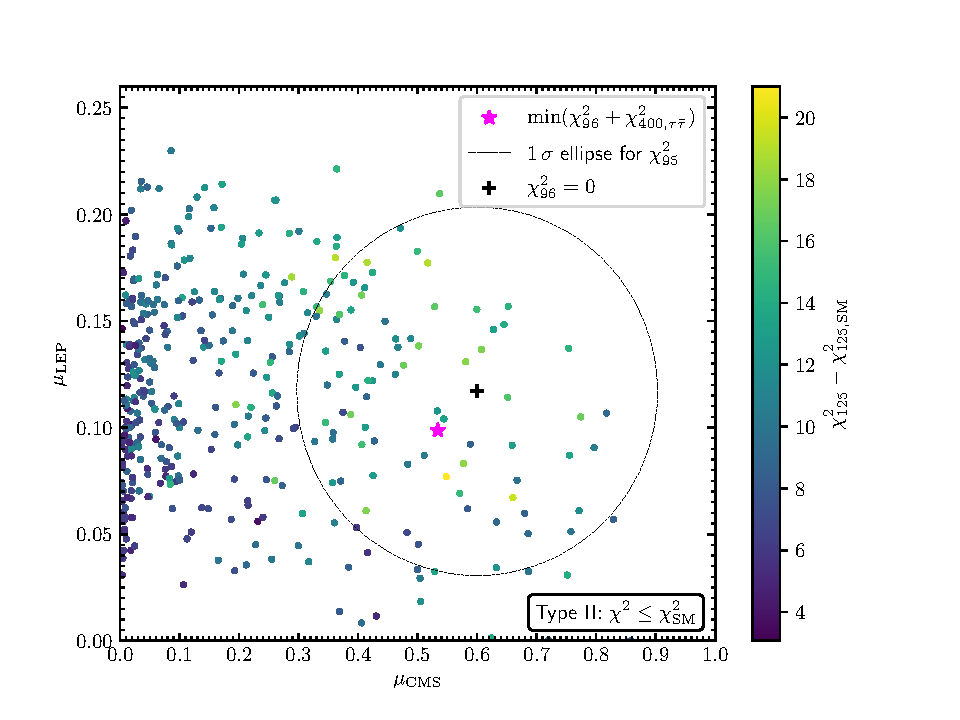
\includegraphics[scale=0.40]{figs/2_hs.pdf} &
			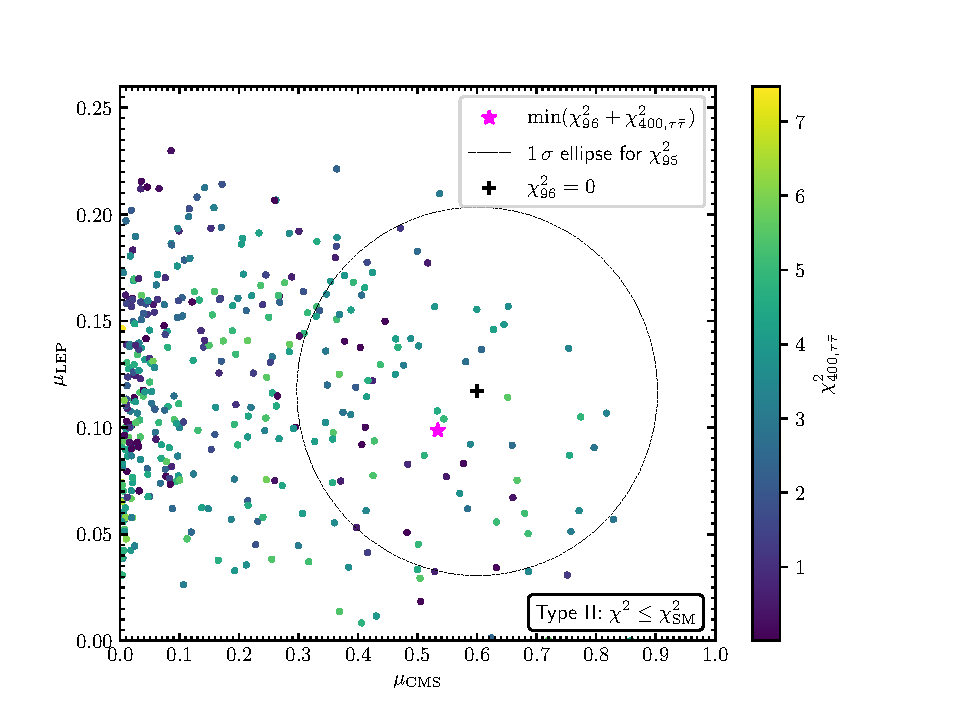
\includegraphics[scale=0.40]{figs/2_ll.pdf}
		\end{tabular}
		\caption{.}
		\label{fig:typeiimu}
	\end{center}
\end{figure}

\begin{figure}[ht!]
	\begin{center}
		\begin{tabular}{cc}
			\centering
			\hspace*{-3mm}
			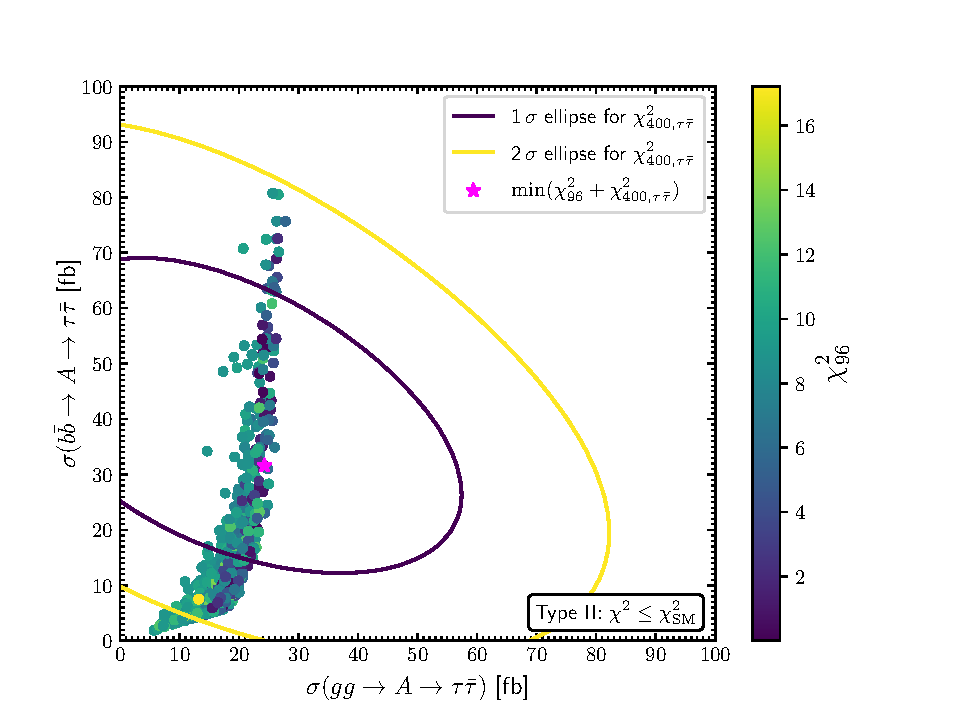
\includegraphics[scale=0.40]{figs/2_LLxs96.pdf} &
			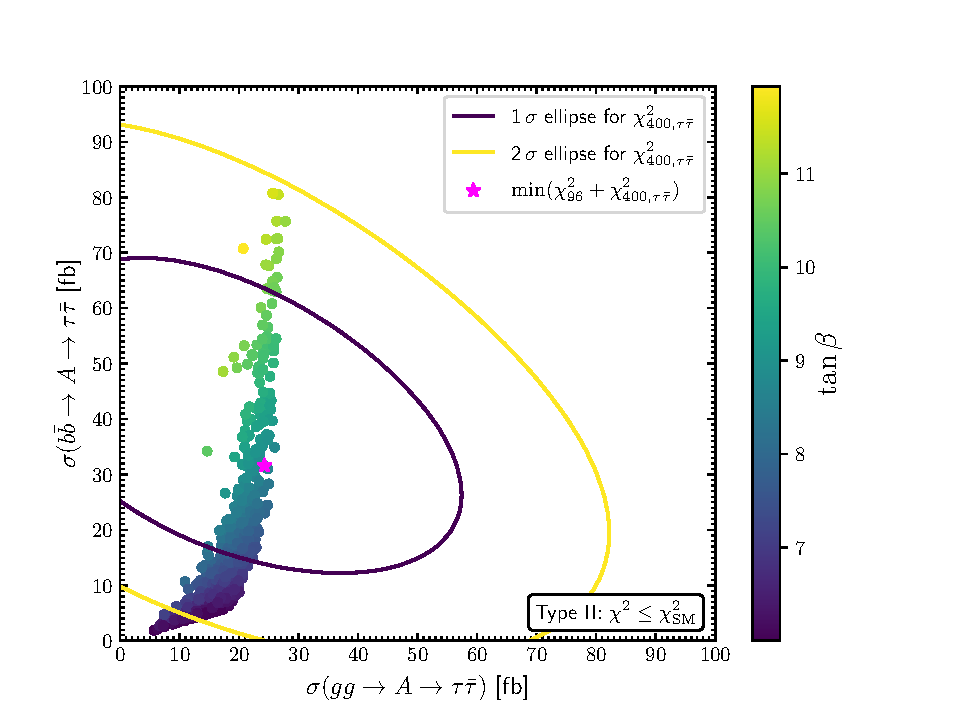
\includegraphics[scale=0.40]{figs/2_LLxstb.pdf}
		\end{tabular}
		\caption{.}
		\label{fig:typeiisigma}
	\end{center}
\end{figure}


\begin{figure}[ht!]
	\begin{center}
		\begin{tabular}{cc}
			\centering
			\hspace*{-3mm}
			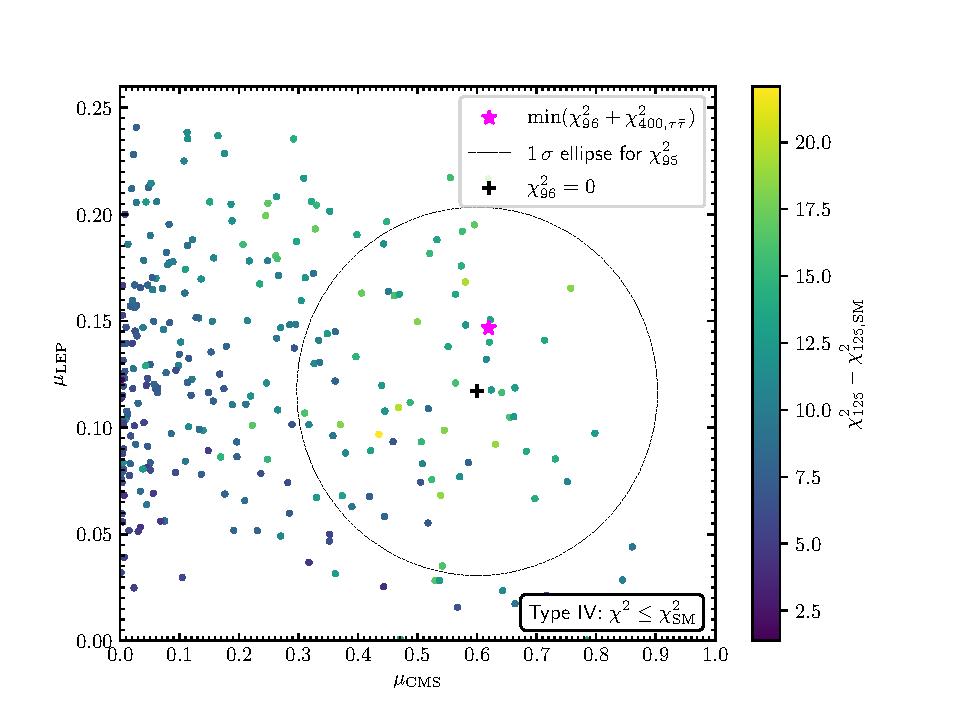
\includegraphics[scale=0.40]{figs/4_hs.pdf} &
			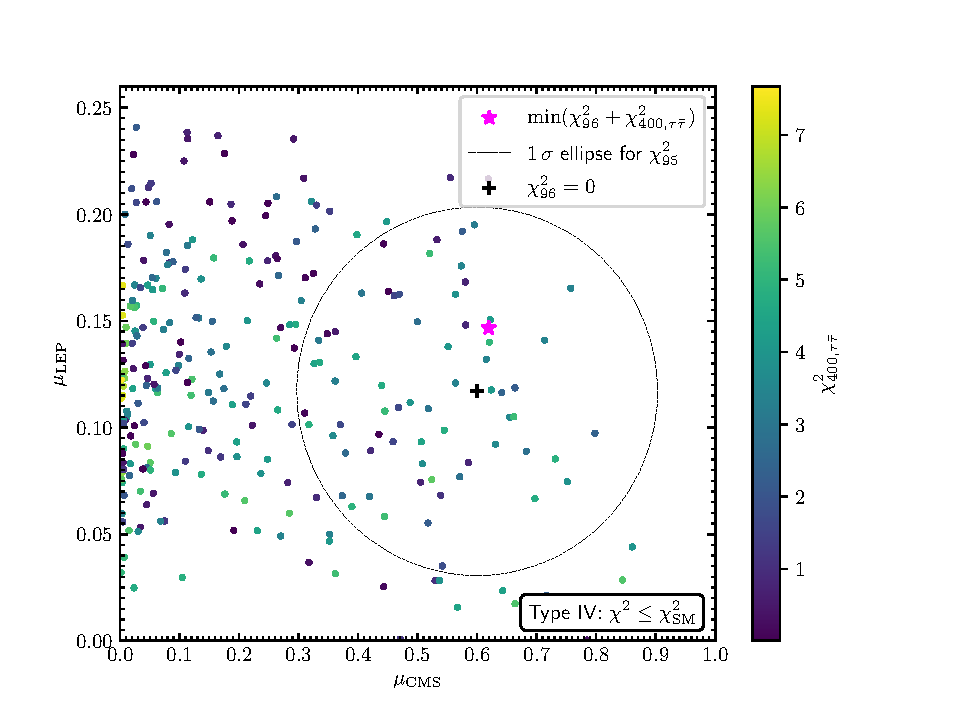
\includegraphics[scale=0.40]{figs/4_ll.pdf}
		\end{tabular}
		\caption{.}
		\label{fig:typeiimu}
	\end{center}
\end{figure}

\begin{figure}[ht!]
	\begin{center}
		\begin{tabular}{cc}
			\centering
			\hspace*{-3mm}
			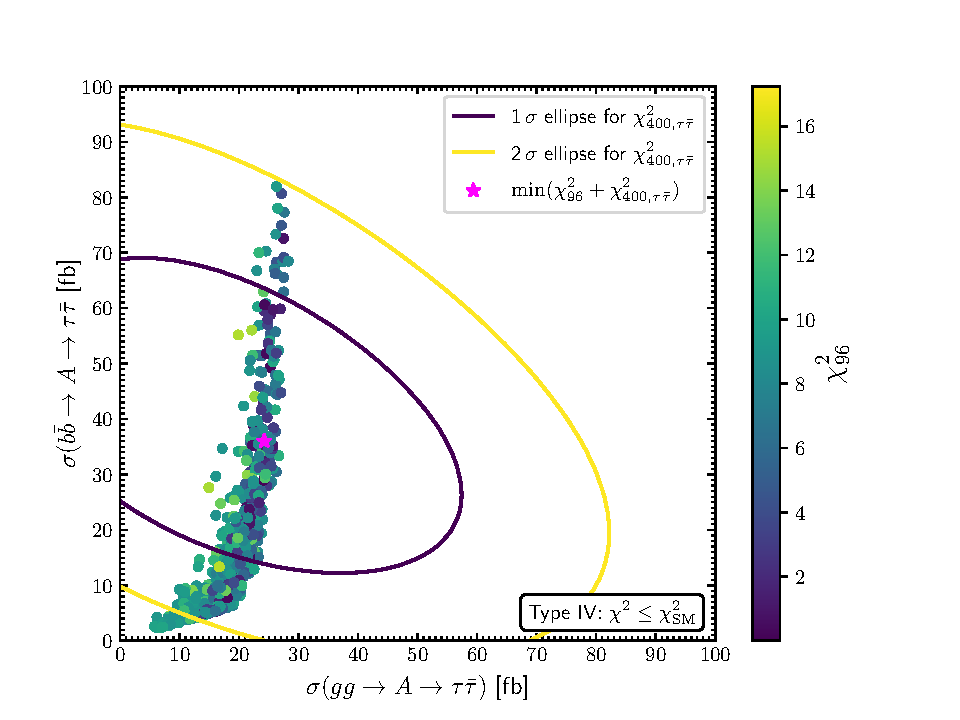
\includegraphics[scale=0.40]{figs/4_LLxs96.pdf} &
			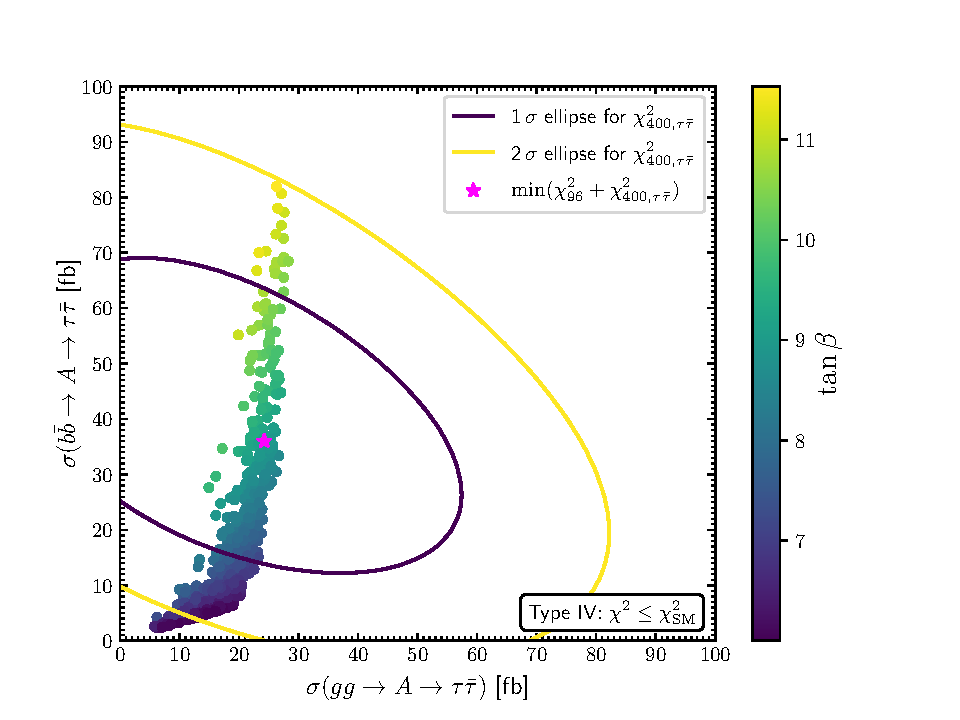
\includegraphics[scale=0.40]{figs/4_LLxstb.pdf}
		\end{tabular}
		\caption{.}
		\label{fig:typeiisigma}
	\end{center}
\end{figure}

%%%%%%%%%%%%%%%%%%%%%%%%%%%%%%%%%%%%%%%%%%%%%%%%%%%%%%%%%%%%%%%%%%%%%%%%%%%%%%%
%%%%%%%%%%%%%%%%%%%%%%%%%%%%%%%%%%%%%%%%%%%%%%%%%%%%%%%%%%%%%%%%%%%%%%%%%%%%%%%


\section{Results}
\label{sec:results}


%%%%%%%%%%%%%%%%%%%%%%%%%%%%%%%%%%%%%%%%%%%%%%%%%%%%%%%%%%%%%%%%%%%%%%%%%%
%%%%%%%%%%%%%%%%%%%%%%%%%%%%%%%%%%%%%%%%%%%%%%%%%%%%%%%%%%%%%%%%%%%%%%%%%%

\section {Conclusions}
\label{sec:conclusion}


%%%%%%%%%%%%%%%%%%%%%%%%%%%%%%%%%%%%%%%%%%%%%%%%%%%%%%%%%%%%%%%%%%%%%%%%%%
%\clearpage

\subsection*{Acknowledgments}

We thank
M.~Kado
for helpful discussions.
The work of S.H.\ is supported in part by the
Spanish Agencia Estatal de Investigaci{\' o}n (AEI) and the EU Fondo Europeo de
Desarrollo Regional (FEDER) through the project FPA2016-78645-P and in part by
the “Spanish Red Consolider MultiDark” FPA2017-90566-REDC, in
part by the MEINCOP Spain under contract FPA2016-78022-P and in part by
the AEI through the grant IFT Centro de Excelencia Severo Ochoa SEV-2016-0597.
  
%%%%%%%%%%%%%%%%%%%%%%%%%%%%%%%%%%%%%%%%%%%%%%%%%%%%%%%%%%%%%%%%%%%%%%%%%%
%%%%%%%%%%%%%%%%%%%%%%%%%%%%%%%%%%%%%%%%%%%%%%%%%%%%%%%%%%%%%%%%%%%%%%%%%%

\begin{appendices}

\section{Derivation of best-fit cross sections and uncertainties}
\label{sec:best-fit-xs}

\subsection{The very simple recipe}
Assuming a gaussian signal, one can extract the expected signal
from the value of the $95\%$ CL exclusion limit $L_{\rm exp}^{95}$
and the corresponding $1\,\sigma$ uncertainty $s_{\rm exp}^{95}$.
The one-sided $95\%$ CL for a normal distribution
lies 1.64 standard deviations from the mean, so that the
central value for the expected signal cross section $\sigma_{\rm exp}$
is given by
\begin{equation}
\sigma_{\rm exp} = L_{\rm exp}^{95} - 1.64 s_{\rm exp}^{95} \, .
\end{equation}
The same is true for the central value of the observed signal
cross section $\sigma_{\rm obs}$. Given the observed $95\%$ CL
exclusion limit $L_{\rm obs}^{95}$ together with the
$1\,\sigma$ uncertainty $s_{\rm obs}^{95}$, and again assuming a gaussian
signal shape, we can write down the relation
\begin{equation}
\sigma_{\rm obs} = L_{\rm obs}^{95} - 1.64 s_{\rm obs}^{95} \, .
\end{equation}
Unfortunately, the uncertainty of the observed signal is not
shown in the plots. However, under the conservative assumption that
\begin{equation}
s_{\rm obs}^{95} = s_{\rm exp}^{95} \, ,
\end{equation}
we can still derive a value for the signal cross section $\sigma_{\rm sig}$,
i.e., the cross section from BSM physics that amounts for the
excess between observed events and expected events based on the
SM hypothesis. In our analysis, $\sigma_{\rm sig}$ is the cross section
given by the NMSSM pseudoscalar and scalar resonances.
Under the assumption that interference of NMSSM contributions and SM
background is negligible, we know that
\begin{equation}
\sigma_{\rm obs} = \sigma_{\rm exp} + \sigma_{\rm sig} \, .
\end{equation}
Thus, we find that $\sigma_{\rm obs}$ is simply given by
the difference between the observed and expected exclusion limits,
\begin{equation}
\sigma_{\rm sig} = L_{\rm obs}^{95} - L_{\rm exp}^{95} \, .
\end{equation}
Note that this definition has the intuitively desired properties.
On the one hand it grows with the number of excess events, and
on the other hand it is exactly zero in case the expected and
the observed exclusion limits coincide, meaning that there is
no excess to be explained by BSM physics.

For the uncertainty of the signal cross section $s_{\rm sig}$
we will assume that it is given by
\begin{equation}
s_{\rm sig} = \frac{s_{\rm exp}^{95}}{1.64} \, ,
\end{equation}
because [insert explanation here].

Based on this simple recipe, we find for the $Zh$ excess the
signal cross sections as shown in \refta{zhsimple}, given for the
mass range in which the excess was observed.
\begin{table}
\centering
\begin{tabular}{l|cc}
$m$ [GeV] & $\sigma_{\rm sig}^{gg}$ [fb] & $\sigma_{\rm sig}^{b \bar b}$ [fb] \\
\hline
400 & $ 89 \pm 33$ & $103 \pm 37$ \\
420 & $118 \pm 27$ & $171 \pm 27$ \\
440 & $114 \pm 23$ & $183 \pm 27$ \\
460 & $ 50 \pm 20$ & $109 \pm 21$ \\
480 & $ 11 \pm 17$ & $ 50 \pm 19$
\end{tabular}
\caption{Signal cross sections for the $Zh$ excess assuming $gg$ production
or $b \bar b$ production as derived following the very simple recipe.}
\label{zhsimple}
\end{table}



\subsection{Advanced approach and its connection to the simple ansatz}

The observed $95\%$ CL exclusion limit on a given cross
section, \sigmaobsnfive, can be used to estimate its
central value. Assuming that the
signal uncertainty is dominated by statistical fluctuations,
i.e. $\sqrt{N_{\rm evt}} = \sqrt{\alpha~\sigmaobsnfive}$, the total
uncertainty reads   
\begin{equation}
\deltaobsnfive = \sqrt {\alpha~\sigmaobsnfive + \deltabkg^2} 
\end{equation}
where \deltabkg denotes the background uncertainty. 
As the one-sided $95\%$ CL of a normal distribution
lies 1.645 standard deviations from its mean the
central value for the expected signal cross section \sigmaobs and its
uncertainty are given by 
\begin{eqnarray} 
\sigmaobs &=& \sigmaobsnfive - 1.645~\deltaobsnfive \label{sigmamarumi} \\
\deltaobs &=& \sqrt{\alpha~\sigmaobs + \deltabkg^2}  \, . \label{deltamarumi}
\end{eqnarray}
In order to estimate $\alpha$ and \deltabkg, we can construct 
the following set of equations 
\begin{eqnarray}
\sigmanfive &=& 1.645~\deltanfive \\ 
\deltanfive^2 &=& \alpha~\sigmanfive + \deltabkg^2 \\
\sigmanfivepone &=& 1.645~\deltanfivepone + \deltabkg \\ 
\deltanfivepone^2 &=& \alpha~\sigmanfivepone + \deltabkg^2 \\
\sigmanfiveptwo &=& 1.645~\deltanfiveptwo + 2~\deltabkg \\ 
\deltanfiveptwo^2 &=& \alpha~\sigmanfiveptwo + \deltabkg^2 \, . 
\end{eqnarray}

Equations~(\ref{sigmamarumi}) and (\ref{deltamarumi}) obtain a very simple form  
if we are assuming that the signal uncertainty can be neglected  
compared to that of the background. In this case, \sigmanfive =
1.645~\deltabkg, and so 
\begin{eqnarray}
\sigmaobs &=& \sigmaobsnfive - \sigmanfive \label{sigmasimple} \\
\deltaobs &=& \deltabkg = \sigmanfive / 1.645  \, . \label{deltasimple}
\end{eqnarray}


%\begin{table}
%\centering
%\begin{tabular}{c|c|c|c|c|c|c|c}
%   & \sigmanfive & \sigmanfivepone & \sigmanfiveptwo & \sigmaobsnfive
%   & \sigmaobs $\pm$ \deltaobs(full) & \sigmaobs
%   $\pm$ \deltaobs (1.645) & \sigmaobs $\pm$ \deltaobs (diff) \\ 
%\hline
%$ ggH\tau\tau$ (ATLAS) & 40.0  & 53.8 & 67.9 & 82.9  & 27.0 $\pm$ 20.5
%& 60.2 $\pm$ 24.3  &  42.9 $\pm$ 13.8 \\
%$ bbH\tau\tau$ (ATLAS) & 30.6  & 41.9 & 54.9 & 77.2  &
%30.6 $\pm$ 18.6  &  58.6 $\pm$ 18.6  &  46.6 $\pm$ 11.3 \\
%$ gg ZH $ (ATLAS) & 139   & 185  & 231 & 228 &  53.5 $\pm$ 56.4 &
%152.3 $\pm$ 84.5 & 89.0 $\pm$ 64.0 \\
%$ bb ZH $ (ATLAS) & 155  & 207  & 258 & 258 & 62.2 $\pm$ 64.1  & 172.5
%$\pm$ 94.2 &  103 $\pm$ 52 \\
%$ top top $  (CMS) &   & & & & & & \\
%\end{tabular}
%
%\caption{Observed signal cross sections for the $\tau\tau$ excesses assuming $gg$ production
%or $b \bar b$ production. All numbers are given in units of fb.}
%\label{zhsimple}
%\end{table}



\begin{table}
\centering
\begin{tabular}{r||c|c|c|c}
   & $ ggH\tau\tau$ (ATLAS) & $ bbH\tau\tau$ (ATLAS) & $ gg ZH $
   (ATLAS) & $ bb ZH $ (ATLAS) \\ 
\hline    
  \sigmanfive [fb] & 40.0 & 30.6 & 139 & 155 \\ 
 \sigmanfivepone [fb] & 53.8 & 41.9 & 185 & 207 \\ 
\sigmanfiveptwo [fb] & 67.9 & 54.9 & 231 & 258 \\ 
 \sigmaobsnfive [fb] & 82.9 & 77.2 & 228 & 258 \\ 
    \sigmaobs $\pm$ \deltaobs(full) [fb] & 27.0 $\pm$ 20.5& 30.6 $\pm$ 18.6
    & 53 $\pm$ 56 & 62 $\pm$ 64 \\  
 \sigmaobs $\pm$ \deltaobs (1.645) [fb] & 60.2 $\pm$ 24.3 & 58.6 $\pm$ 18.6
    & 152 $\pm$ 85 & 173 $\pm$ 94 \\ 
 \sigmaobs $\pm$ \deltaobs (diff) [fb] & 42.9 $\pm$ 13.8 & 46.6 $\pm$ 11.3
    & 89 $\pm$ 64 & 103 $\pm$ 52 \\ 
 \sigmaobs $\pm$ \deltaobs (georg) [fb] & 30.3 $\pm$ 22.2  &  34.3
    $\pm$ 19.3  & 60.6 $\pm$  65.6 & 70.6 $\pm$ 74.2 \\ 
\end{tabular}

\caption{Observed signal cross sections} 
\label{obsignal}
\end{table}

\end{appendices}


%%%%%%%%%%%%%%%%%%%%%%%%%%%%%%%%%%%%%%%%%%%%%%%%%%%%%%%%%%%%%%%%%%%%%%%%%%%%%%%
%%%%%%%%%%%%%%%%%%%%%%%%%%%%%%%%%%%%%%%%%%%%%%%%%%%%%%%%%%%%%%%%%%%%%%%%%%%%%%%


\newcommand\jnl[1]{\textit{\frenchspacing #1}}
\newcommand\vol[1]{\textbf{#1}}

\begin{thebibliography}{100}

%\input{ref}

\bibitem{CidVidal:2018eel}
X.~Cid Vidal \textit{et al.}, 
CERN Yellow Rep. Monogr. \textbf{7} (2019), 585-865
[arXiv:1812.07831 [hep-ph]].

\bibitem{Chen:2013jvg}
C.~Y.~Chen, M.~Freid and M.~Sher,
``Next-to-minimal two Higgs doublet model,''
Phys. Rev. D \textbf{89} (2014) no.7, 075009
doi:10.1103/PhysRevD.89.075009
[arXiv:1312.3949 [hep-ph]].

\bibitem{Muhlleitner:2016mzt}
M.~Muhlleitner, M.~O.~P.~Sampaio, R.~Santos and J.~Wittbrodt,
``The N2HDM under Theoretical and Experimental Scrutiny,''
JHEP \textbf{03} (2017), 094
doi:10.1007/JHEP03(2017)094
[arXiv:1612.01309 [hep-ph]].


\end{thebibliography}



%%%%% CLEAR DOUBLE PAGE!
\newpage{\pagestyle{empty}\cleardoublepage}

%%%%%%%%%%%%%%%%%%%%%%%%%%%%%%%%%%%%%%%%%%%%%%%%%%%%%%%%%%%%%%%%%%%%%%%%%%%

\end{document}
